\chapter{Exercise 4}
\label{chap:4}
The topic of this chapter is the evaluation ofthe collected data from Chapter \ref{chap:3}. For this the data shown at \ref{appendix:output} is used.

\section{Time to read line}
This section analysis the time needed to read a single line. For this the Loadtimes per line were divided by the class, as longer lines (line class equal to length) took linearly longer. As seen in figure \ref{fig:load_class_point} the loadingtimes bummped at a length of ten points or more. To further investigate this, the timings for \texttt{getX()} and \texttt{getY()} were looked at (see figure \ref{fig:getY_getX}). This showed the reason for the longer loading times for lines with more than ten points. \texttt{getY()} takes one extra millisecond for each call after the ninth point. This corresponds to the one millisecond more that is needed to load such lines.

\begin{figure}[h!]
    \begin{center}
        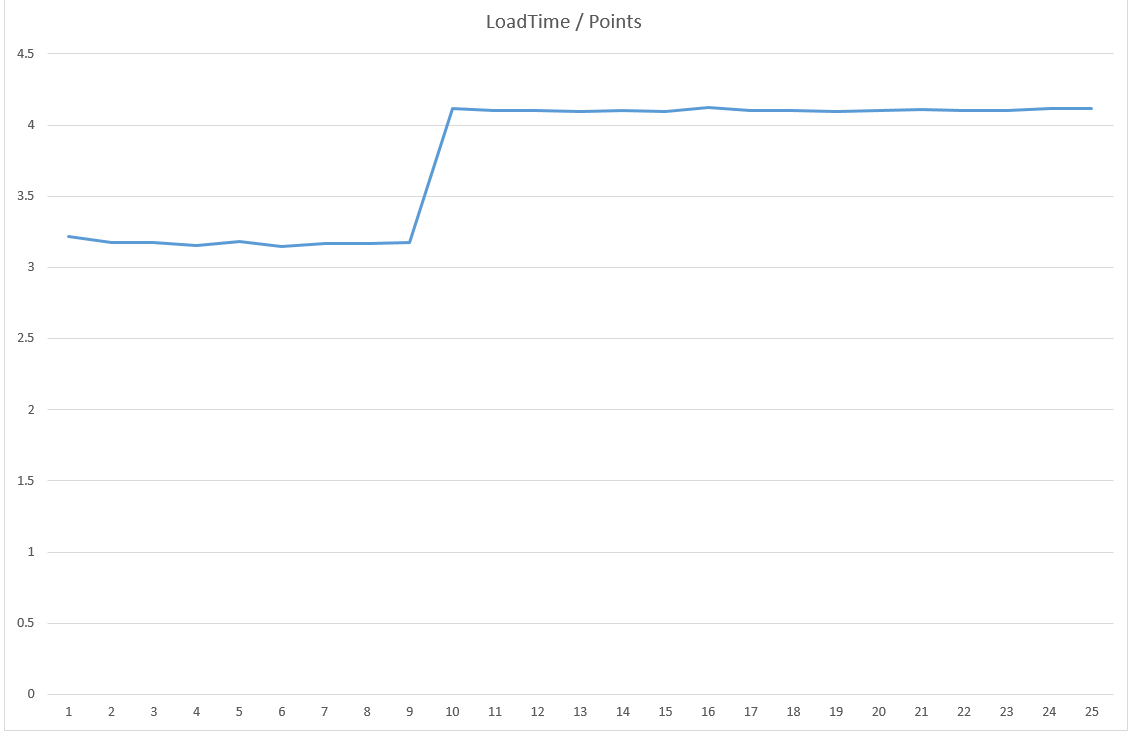
\includegraphics[width=0.99\textwidth]{img/loadingtime_class_point_avg.png}
        \caption{Loading times per line class (avg) divided by line class to accomendad for linear factor}
        \label{fig:load_class_point}
    \end{center}
\end{figure}

\begin{figure}[h!]
    \begin{center}
        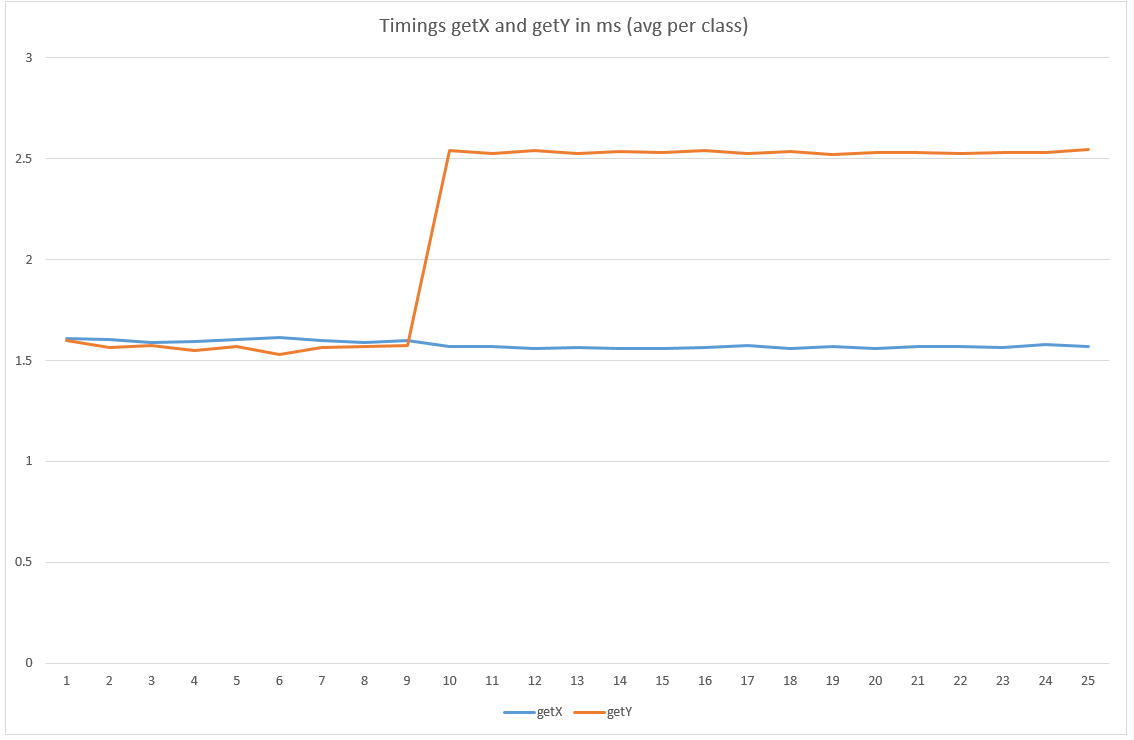
\includegraphics[width=0.99\textwidth]{img/getx_gety.png}
        \caption{Timings getX and getY for each line class}
        \label{fig:getY_getX}
    \end{center}
\end{figure}

\section{Timings slope and intercept}
For the analysis of calls to \texttt{slope()} and \texttt{intercept()} the uncached timings were used. The figure \ref{fig:slope_intercept} shows the measured timings for each line class. For line class one the calls need especially long, since those are not valid and slope throws an exception. This process is especially expensive on compute time and is measured with the current implementation. Also observable is the behaivour for 12 to 13 points, where the calls are faster for more points. This might be since the Java JVM optimizations kick in and optimize the performance. Also, this diagram shows that for \texttt{slope()} the caching algorith works fine, as \texttt{slope()} is called in \texttt{intercept()} but does not seem to add any amount of execution time to the call.

\begin{figure}[h!]
    \begin{center}
        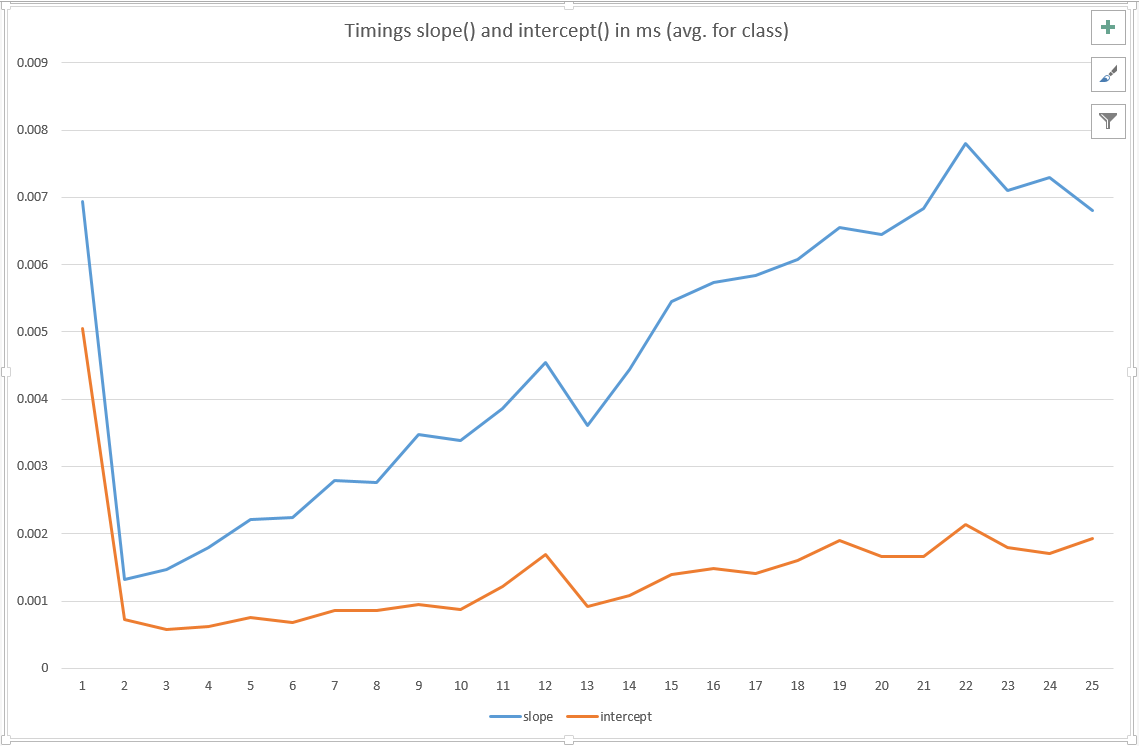
\includegraphics[width=0.99\textwidth]{img/slope_intercept_avg.png}
        \caption{Timings slope and intercept}
        \label{fig:slope_intercept}
    \end{center}
\end{figure}
